\begin{figure}[t!]
    \centering
    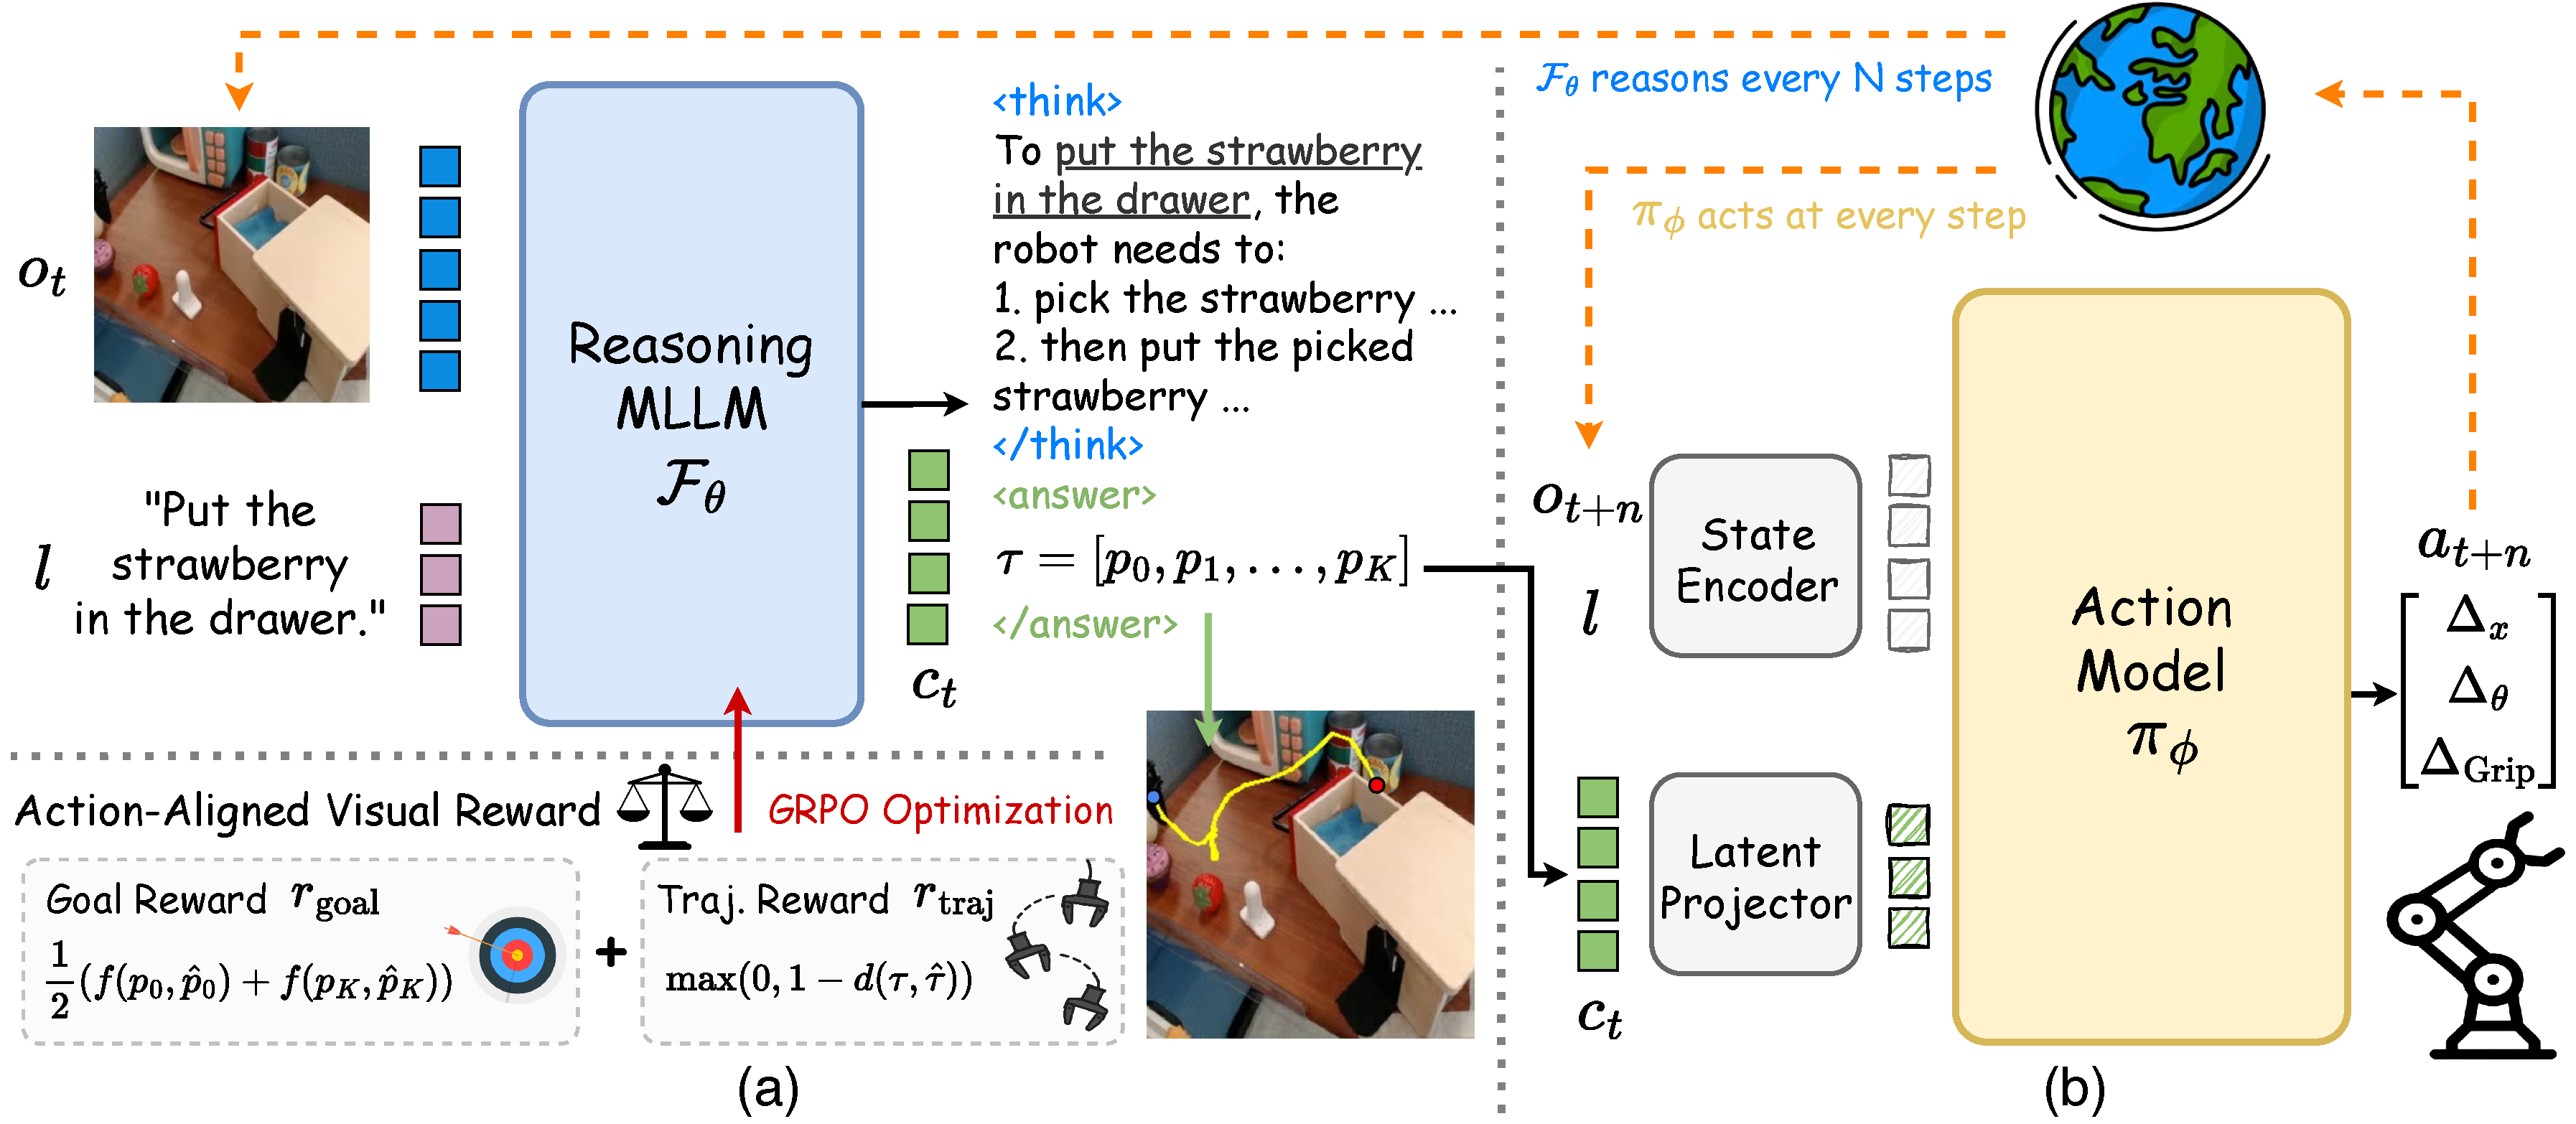
\includegraphics[width=1.0\linewidth]{figures/images/overview.pdf}
    \caption{\textbf{Overview of our \ours{}.} (a) Given observation $o_t$ and instruction $l$, \ours{} advances \emph{action-aligned} rewards derived from visual trajectory $\tau$ to incentivize embodied reasoning capability of Reasoning MLLM $\mathcal{F}_\theta$. (b) Conditioned on the visual plan latent $c_t$, the DiT-based Action Model $\pi_\phi$ learns to predict executable action while keeping $\mathcal{F}_\theta$ frozen. Note that, during inference, $\pi_\phi$ and $\mathcal{F}_\theta$ could operate asynchronously to enable slow thinking and fast control for VLA reasoning tasks.}
    \label{fig:overview}
\end{figure}